\documentclass{article}

\usepackage[dvips]{graphicx}

\begin{document}

\title{A primer on data structures for machine learning}

\maketitle

\section{Introduction}

So you�ve decided to move beyond canned algorithms and start to code your own machine learning methods. Maybe you�ve got an idea for a cool new way of clustering data, or maybe you are frustrated by the limitations in your favorite statistical classification package.
    In either case, the better your knowledge of data structures and algorithms, the easier time you�ll have when it comes time to code up.

I don�t think the data structures used in machine learning are significantly different than those used in other areas of software development. Because of the size and difficulty of many of the problems, however, having a really solid handle on the basics is essential.
Also, because machine learning is a very mathematical field, one should have in mind how data structures can be used to solve mathematical problems and as mathematical objects in their own right.

    There are two ways to classify data structures: by their implementation and by their operation.
By implementation, I mean the nuts and bolts of how they are programmed and the actual storage patterns. How they look on the outside is less important than what�s going on under the hood. For data structures classed by operation or 
{\it abstract data types}, it is the opposite: their external appearance and operation is more important than how they are implemented, and in fact they can usually be implemented using a number of different internal representations.

\section{Arrays}

I�m not kidding when I say that the basic array is the most important data structure in machine learning, and there is more to this bread-and-butter type than you might think. Arrays are important because they are used in linear algebra: the most useful and powerful mathematical tool at your disposal.

Therefore, the most common types will be the one- and two-dimensional variety, corresponding to vectors and matrices respectively, but you will occasionally encounter three- or four-dimensional arrays either for higher ranked tensors or to group examples of the former.

When doing matrix arithmetic, you will have to choose from a dizzying variety of libraries, data types, and even languages. Many scientific programming languages such as Matlab, Interactive Data Language (IDL), and Python with the Numpy extension are designed primarily for working with vectors and matrices.

But the nice thing about these data structures is that, even in more general-purpose programming languages, implementing vectors and matrices is straightforward right next to the metal, assuming the language has any Fortran DNA in it at all. Consider the translation of matrix-vector multiplication:
\begin{eqnarray}
\vec y & = & A \vec x \\
y_i = \sum_{i=0}{n} a_{ij} x_j
\end{eqnarray}
into C++:
\begin{verbatim}
for (int i=0; i<n; i++) {
  y[i]=0;
  for (int j=0; j<n; j++) y[i]+=a[i][j]*x[j]
}
\end{verbatim}

\section{Extensible array}

\begin{figure}
\includegraphics[width=0.9\textwidth]{extensible_array}
\caption{Typical storage pattern of an extensible array.}
\end{figure}

In most cases, arrays can be allocated to a fixed size at run time, or you can calculate a reliable upper bound. In those cases where you need your arrays to expand indefinitely, you can use an extensible array such as the vector class in the C++ standard template library (STL). Regular arrays in Matlab are similarly extensible, and extensible arrays are the basis of the entire Python language.

In this data structure, there are two pieces of ``meta-data'' stored alongside the actual data values. These are the amount of storage space allocated to the data structure and the actual size of the array. As soon as the size of the array exceeds the storage space, a new space is allocated that�s twice the size, the values copied into it, and the old array deleted.

This is an $O(n)$ operation, where n is the size of the array, but since it only happens occasionally, time to add a new value onto the end actually amortizes to constant time, $O(1)$. It is a very flexible data structure with fast average insertions and fast access.

Extensible arrays are excellent for composing other, more complex data structures and making them extensible. For example, to store a sparse matrix: any number of new elements can be added onto the end and they are then sorted by position to make location faster. More on this later.

\section{Linked list}

\begin{figure}
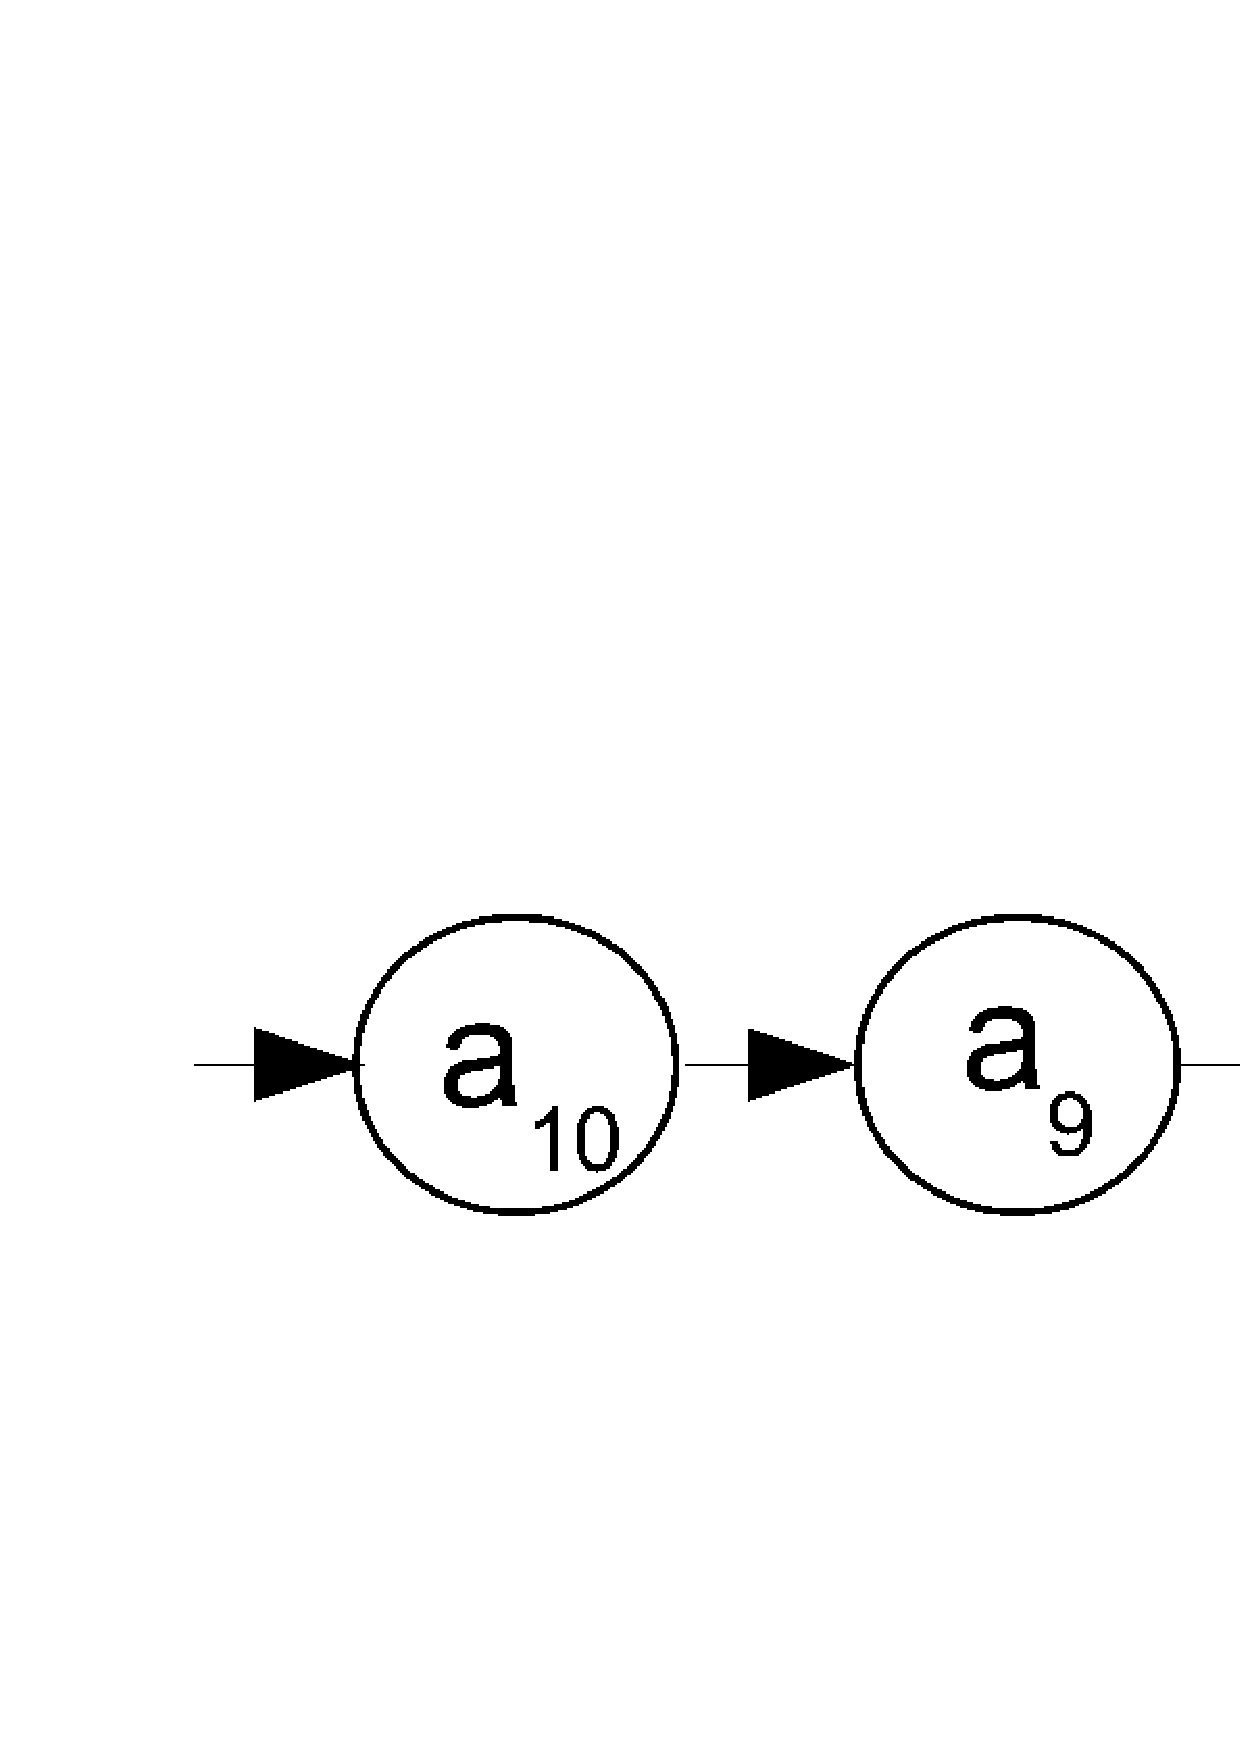
\includegraphics[width=0.9\textwidth]{linked_list}
\caption{Storage layout for a linked list.}
\end{figure}

A linked list consists of several separately allocated nodes. Each node contains a data value plus a pointer to the next node in the list. Insertions, at constant time, are very efficient, but accessing a value is slow and often requires scanning through much of the list.

Linked lists are easy to splice together and split apart. There are many variations: for instance, insertions can be done at either the head or the tail; the list can be doubly-linked and there are many similar data structures based on the same principle such as the binary tree, below.

Mainly, I find linked lists useful for parsing lists of indeterminate length. Afterwards, they can be converted to fixed-length arrays for fast access. For this reason, I use a linked list class that includes a method for conversion to an array.

\section{Binary tree}

\begin{figure}
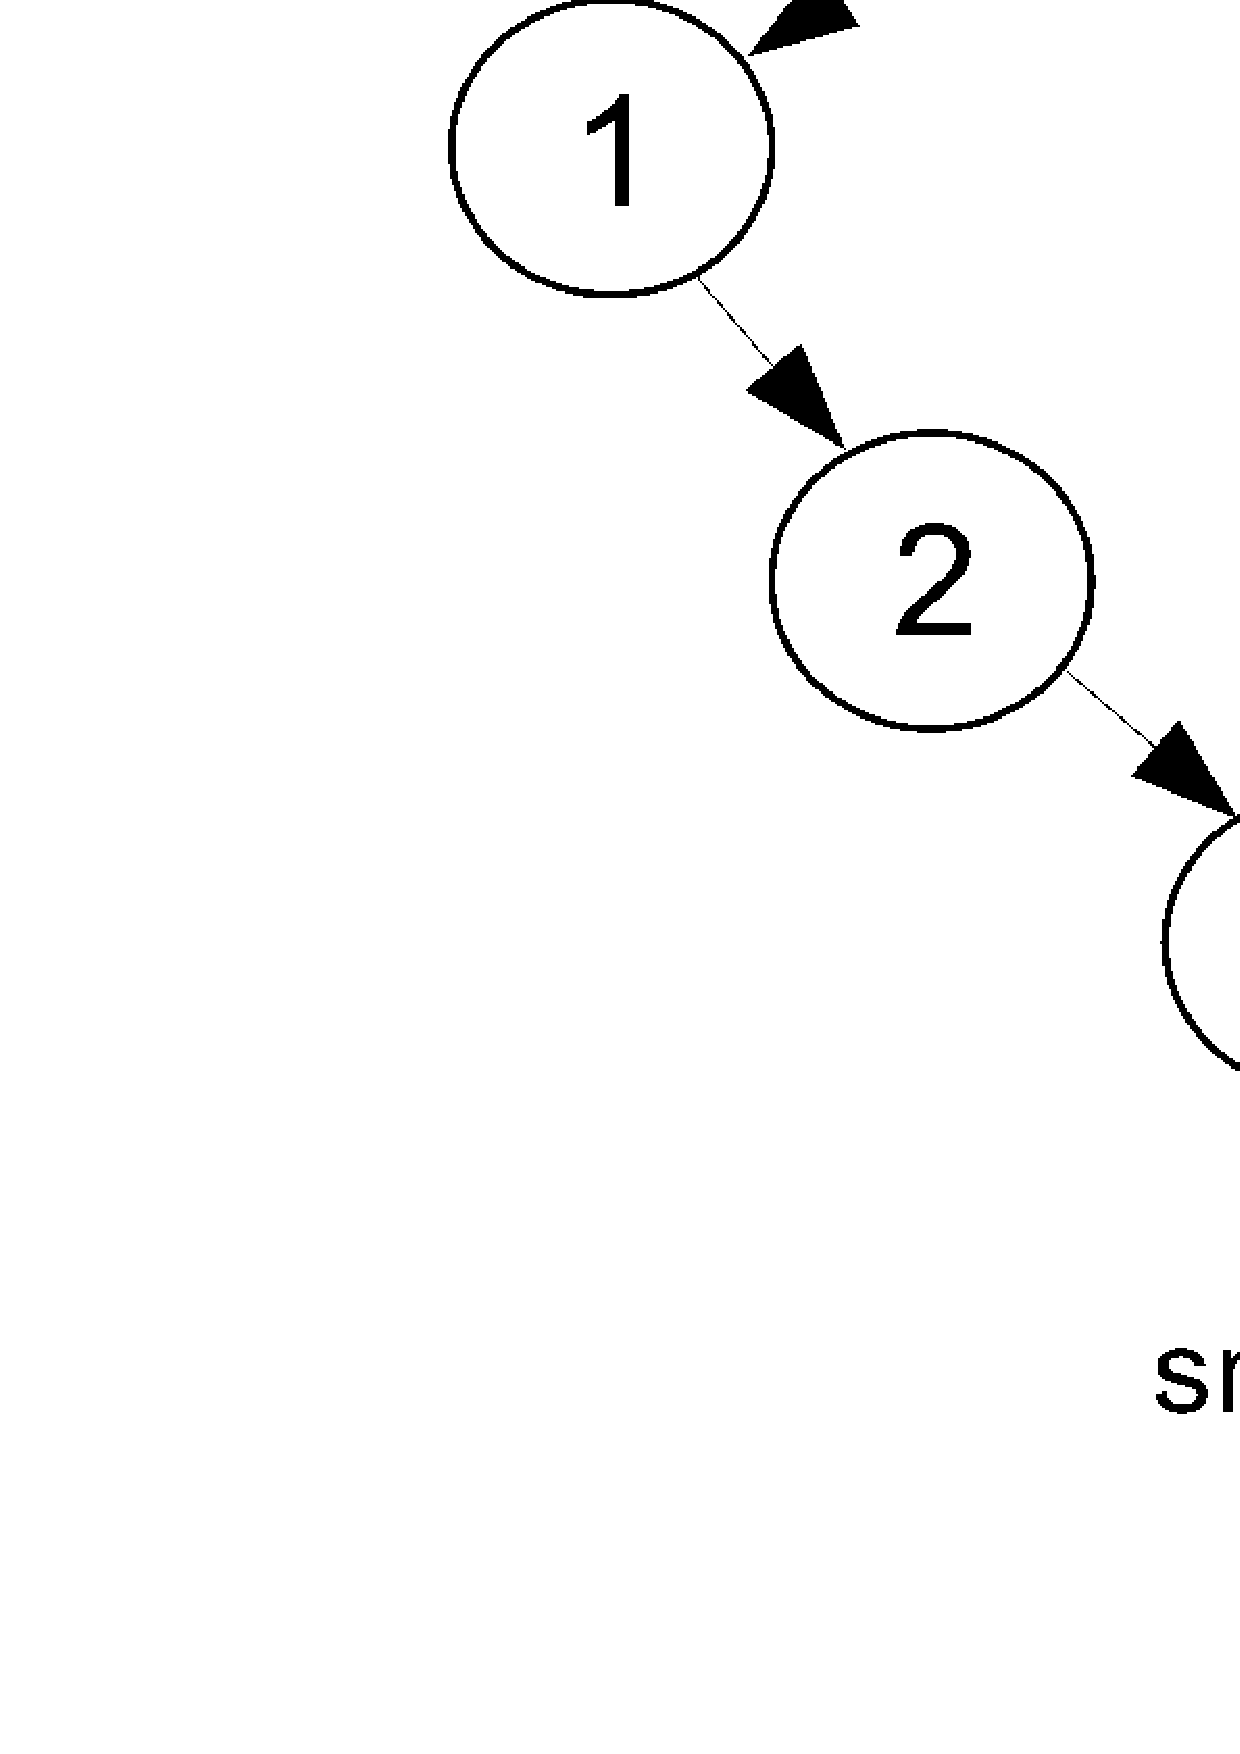
\includegraphics[width=0.9\textwidth]{tree}
\caption{Storage pattern for a sorted binary tree.}
\end{figure}

A binary tree is similar to a linked list except that each node has two pointers to subsequent nodes instead of just one. The value in the left child is always less than the value in the parent node, which in turn is smaller than that of the right child. Thus, data in binary trees is automatically sorted. Both insertion and access are efficient at $O(log n)$ on average. Like linked lists, they are easy to transform into arrays and this is the basis for a tree-sort.

\section{Balanced tree}

\begin{figure}
\includegraphics[width=0.9\textwidth]{tree2}
\caption{Balancing a binary tree.}
\end{figure}

If the data is already already sorted, binary trees are less efficient at O(n) worst case since the data will be laid out linearly as if it were a linked list. While the ordering in a binary tree is constrained, it is by no means unique and the same list can be arranged in many different configurations depending on the order in which it is inserted.

There are several transformations that can be applied to a tree in order to make it more balanced. Self-balancing trees perform these operations automatically in order to keep access and insertion at an optimal average.

\section{Heap}

\begin{figure}
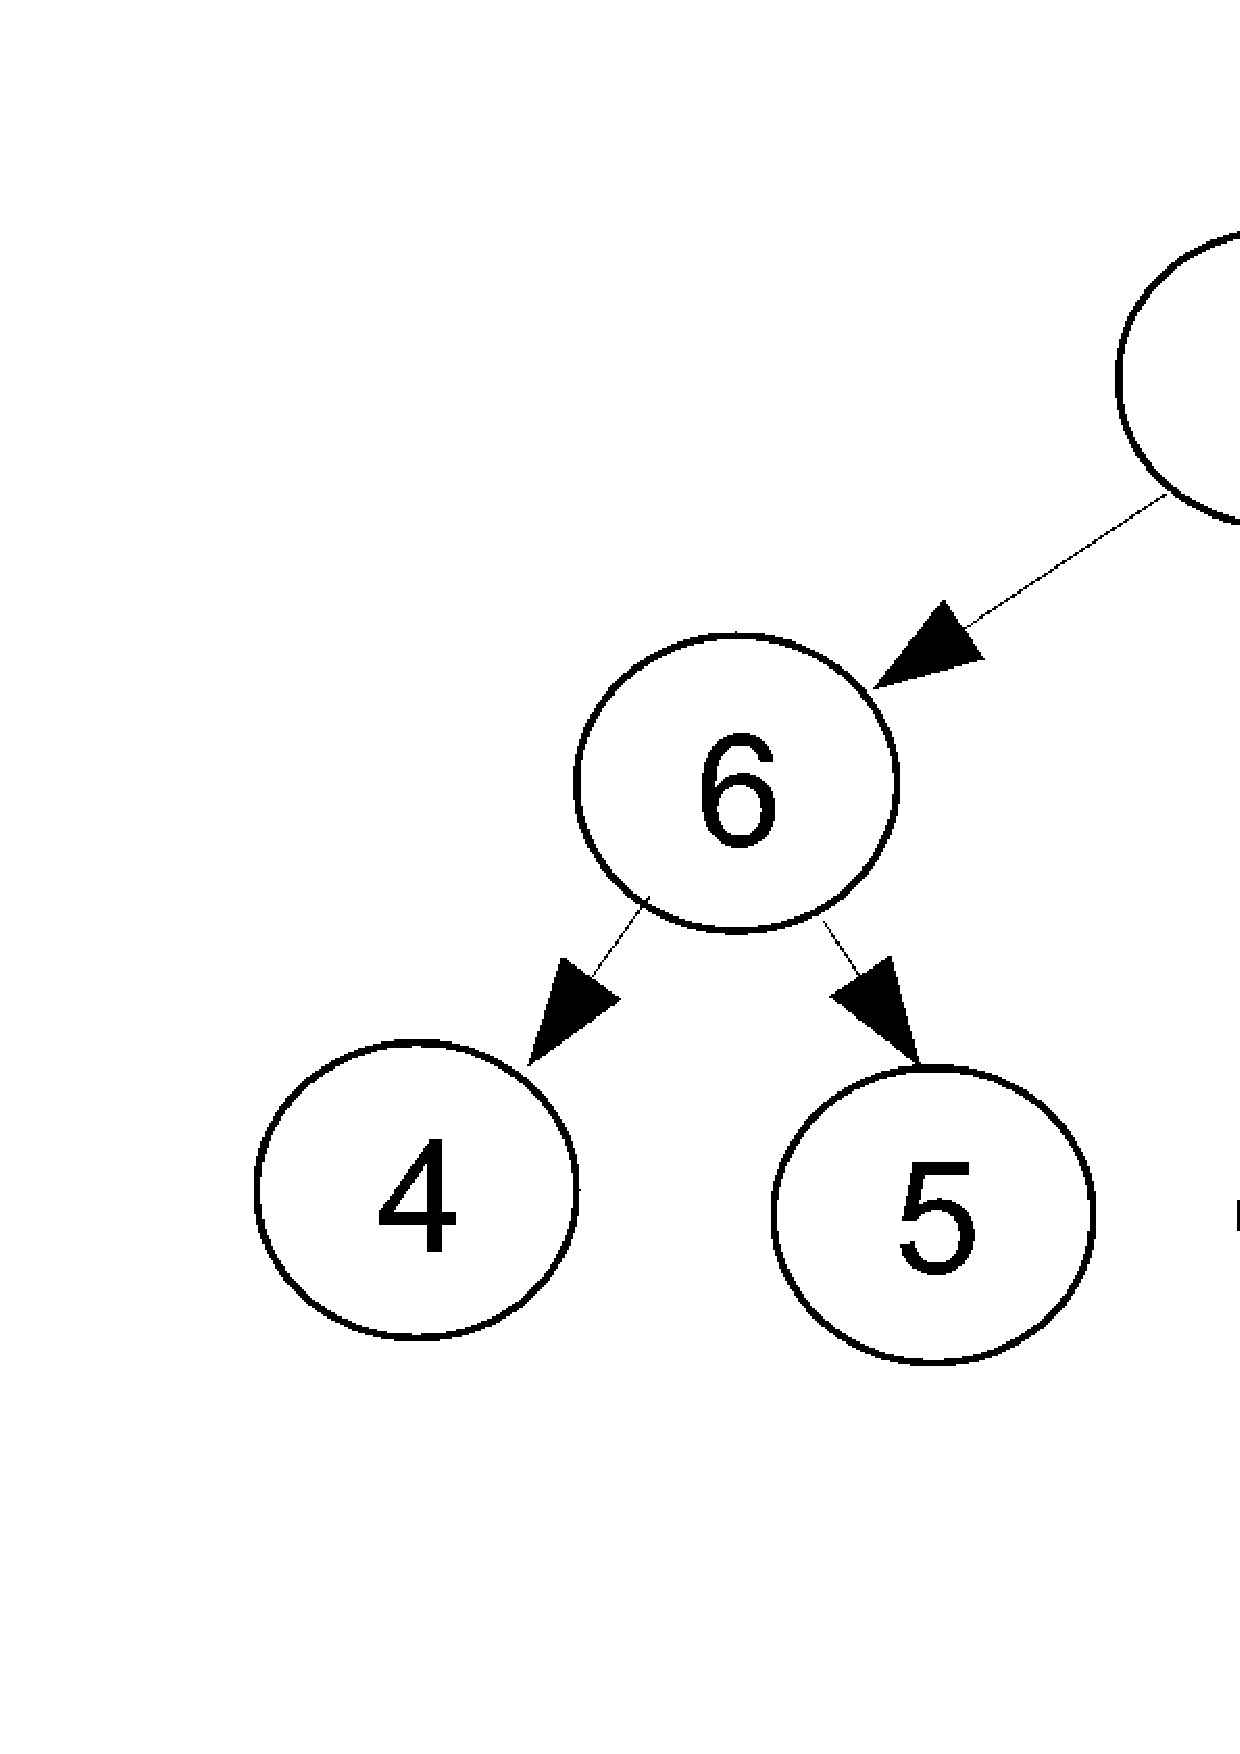
\includegraphics[width=0.9\textwidth]{heap}
\caption{Diagram of a heap.}
\end{figure}

A heap is another hierarchical, ordered data structure similar to a tree except instead of a horizontal ordering, it has a vertical ordering. This ordering applies along the hierarchy, but not across it: the parent is always larger than both its children, but a node of higher rank is not necessarily larger than a lower one that�s not directly beneath it.

Both insertion and retrieval are performed by promotion. An element is first inserted in the highest available position. Then it is compared with its parent and promoted until it reaches the right rank. To take an element off the heap, the larger of the two children is promoted to the missing position, then the larger of those two children is promoted and so on until everything has trickled up the ranks.

Typically, the highest ranking value at the top is pulled off the heap in order to sort a list. Unlike a tree, most heaps are simply stored in an array with the relationships between elements only implicit.

\section{Stack}

A stack is defined as ``first in, last out.'' An element is pushed onto the top of the stack where it covers the previous element. The top element must be popped off before any of the others can be accessed.
    Stacks are mainly useful for parsing grammars and implementing computer languages.

There are many machine learning applications for which a domain specific language (DSL) is the perfect solution. For instance, the libAGF library uses a recursive control language to generalize binary classification to multi-class. A special character is used to repeat a previous option, but because the language is recursive, the option must be taken from the same hierarchical level or higher. This is implemented by a stack.

\section{Queue}

A queue is defined as ``first in, first out.'' Think of the line at the bank teller (for those of us still old enough to remember a time before internet banking). Queues are useful in real time programming so that the program can maintain a list of jobs to be processed.

Consider an application to record split times of athletes. You type in the bib number and hit enter, except in the time it took you to do that the next athlete behind has also passed. So you type in a list of bib numbers of the nearest approaching athletes, then hit a separate key to register the next in the queue as having passed.

\section{Associative array}

In an associative array, there are two types of data which are stored in pairs: the key and its associated value. The data structure is relational in nature: the value is addressed by its key. Since much of the training data is also relational, this type of data structure would seem ideally suited to machine learning problems.
In practice, it�s not used so much, in part because most associative arrays are only one-dimensional, whereas machine learning data is typically multi-dimensional. 

Associative arrays are good for building dictionaries.
Suppose you are building a DSL, want to store a list of functions and variables, and need to distinguish between the two.
\begin{eqnarray*}
 ``sin'' & \rightarrow & function \\
 ``var'' & \rightarrow & variable \\
 ``exp'' & \rightarrow & function \\
 ``x'' & \rightarrow & variable \\
 ``sqrt'' & \rightarrow & function \\
 ``a'' & \rightarrow & variable
\end{eqnarray*}

Querying the array on ``sqrt'' would return, ``function.''

\section{Custom data structures}

As you work on more problems, you are sure to encounter those for which the standard recipe box does not contain optimal structures. You will need to design your own data structure.

Consider a multi-class classifier, which generalizes a binary classifier to work with classification problems having more than two classes. An obvious solution is bisection: recursively split the classes into two groups. You could use something similar to a binary tree to organize the binary classifiers, except that a hierarchical solution is not the only method of solving for multi-class.
    Consider several partitions that are then used to solve for all the class probabilities simultaneously.
The most general solution would combine the two, thus each hierarchical partition need not be binary but could be solved by a non-hierarchical multi-class classifier. This is the approach taken in the libAGF library.

More complex data structures can also be composed of the basic structures. Consider a sparse matrix class. In a sparse matrix, most of the elements are zero and only the non-zero elements are stored. We could store the position and value for each element as a triplet and have a list of them in an extensible array.

Consider the 3 by 3 identity:
\begin{equation}
I = \left [ \begin{array}{l}
	\lbrace 1, 1, 1. \rbrace\\
	\lbrace 2, 2, 1. \rbrace\\
	\lbrace 3, 3, 1. \rbrace
\end{array}
\right ]
\end{equation}

\section{Conclusion}

Data structures are only occasionally interesting in their own right. What makes them truly interesting are the kinds of problems you can solve with them.

For most of the work I do, I�m using a lot of basic fixed-length arrays. I mostly use more sophisticated data structures to make the programs a little smoother in how they run and interface with the outside world and a little more user friendly. Less like the Fortran programs of yore where you had to endure a compile cycle of close to half an hour just to change the grid sizes (I actually worked on a program like this!).

Even if you can�t come up with an application off the top of your head I still I think it�s good to know about things like stacks and queues. You never know when one might come in handy.
Really sophisticated artificial intelligence applications might use things like directed and undirected graphs, which are really just generalizations of trees and linked lists. How are you going to build things like the former if you can�t cope with the latter?

\section{Problems}

f you want to practice and realize data structures for ML algorithm yourself, try to solve some of problems below:
\begin{enumerate}
\item Encapsulate the matrix-vector multiplication code snippet into a subroutine called \verb/matrix_times_vector/. Design the calling syntax for the subroutine.
\item Using \verb/struct/, \verb/typedef/ or \verb/class/, encapsulate both vectors and matrices into a pair of abstract types called \verb/vect/ and \verb/matrix/, respectively. Design an API for the types.
\item Find at least three libraries online that do the above.
\item Download and install the LIBSVM library. Consider the method \verb/Kernel::k_function/ on line 316 of ``svm.cpp''. What are the advantages and disadvantages of the data structure used to hold vectors?
\item How would you re-factor calculation of kernel functions in the LIBSVM library?
\item Which data structures described in the text are abstract types?
\item What internal representation or data structure could you use to implement the abstract data types? Are there any that are not included in the list above?
\item Using a binary tree, design an associative array.
\item Consider the vector type in LIBSVM. How can this be used to represent a sparse matrix? Contrast this with the sparse matrix class described above. Look at the complete type. What are the advantages and disadvantages of each representation?
\item Implement a treesort and a heapsort. Now use the same data structures to find the top $k$ elements. What common machine learning algorithm is this good for?
\item Implement your favorite data structure in your favourite language.
\end{enumerate}

\end{document}


